% Options for packages loaded elsewhere
\PassOptionsToPackage{unicode}{hyperref}
\PassOptionsToPackage{hyphens}{url}
\PassOptionsToPackage{dvipsnames,svgnames,x11names}{xcolor}
%
\documentclass[
  letterpaper,
  DIV=11,
  numbers=noendperiod]{scrartcl}

\usepackage{amsmath,amssymb}
\usepackage{iftex}
\ifPDFTeX
  \usepackage[T1]{fontenc}
  \usepackage[utf8]{inputenc}
  \usepackage{textcomp} % provide euro and other symbols
\else % if luatex or xetex
  \usepackage{unicode-math}
  \defaultfontfeatures{Scale=MatchLowercase}
  \defaultfontfeatures[\rmfamily]{Ligatures=TeX,Scale=1}
\fi
\usepackage{lmodern}
\ifPDFTeX\else  
    % xetex/luatex font selection
\fi
% Use upquote if available, for straight quotes in verbatim environments
\IfFileExists{upquote.sty}{\usepackage{upquote}}{}
\IfFileExists{microtype.sty}{% use microtype if available
  \usepackage[]{microtype}
  \UseMicrotypeSet[protrusion]{basicmath} % disable protrusion for tt fonts
}{}
\makeatletter
\@ifundefined{KOMAClassName}{% if non-KOMA class
  \IfFileExists{parskip.sty}{%
    \usepackage{parskip}
  }{% else
    \setlength{\parindent}{0pt}
    \setlength{\parskip}{6pt plus 2pt minus 1pt}}
}{% if KOMA class
  \KOMAoptions{parskip=half}}
\makeatother
\usepackage{xcolor}
\setlength{\emergencystretch}{3em} % prevent overfull lines
\setcounter{secnumdepth}{5}
% Make \paragraph and \subparagraph free-standing
\ifx\paragraph\undefined\else
  \let\oldparagraph\paragraph
  \renewcommand{\paragraph}[1]{\oldparagraph{#1}\mbox{}}
\fi
\ifx\subparagraph\undefined\else
  \let\oldsubparagraph\subparagraph
  \renewcommand{\subparagraph}[1]{\oldsubparagraph{#1}\mbox{}}
\fi


\providecommand{\tightlist}{%
  \setlength{\itemsep}{0pt}\setlength{\parskip}{0pt}}\usepackage{longtable,booktabs,array}
\usepackage{calc} % for calculating minipage widths
% Correct order of tables after \paragraph or \subparagraph
\usepackage{etoolbox}
\makeatletter
\patchcmd\longtable{\par}{\if@noskipsec\mbox{}\fi\par}{}{}
\makeatother
% Allow footnotes in longtable head/foot
\IfFileExists{footnotehyper.sty}{\usepackage{footnotehyper}}{\usepackage{footnote}}
\makesavenoteenv{longtable}
\usepackage{graphicx}
\makeatletter
\def\maxwidth{\ifdim\Gin@nat@width>\linewidth\linewidth\else\Gin@nat@width\fi}
\def\maxheight{\ifdim\Gin@nat@height>\textheight\textheight\else\Gin@nat@height\fi}
\makeatother
% Scale images if necessary, so that they will not overflow the page
% margins by default, and it is still possible to overwrite the defaults
% using explicit options in \includegraphics[width, height, ...]{}
\setkeys{Gin}{width=\maxwidth,height=\maxheight,keepaspectratio}
% Set default figure placement to htbp
\makeatletter
\def\fps@figure{htbp}
\makeatother
\newlength{\cslhangindent}
\setlength{\cslhangindent}{1.5em}
\newlength{\csllabelwidth}
\setlength{\csllabelwidth}{3em}
\newlength{\cslentryspacingunit} % times entry-spacing
\setlength{\cslentryspacingunit}{\parskip}
\newenvironment{CSLReferences}[2] % #1 hanging-ident, #2 entry spacing
 {% don't indent paragraphs
  \setlength{\parindent}{0pt}
  % turn on hanging indent if param 1 is 1
  \ifodd #1
  \let\oldpar\par
  \def\par{\hangindent=\cslhangindent\oldpar}
  \fi
  % set entry spacing
  \setlength{\parskip}{#2\cslentryspacingunit}
 }%
 {}
\usepackage{calc}
\newcommand{\CSLBlock}[1]{#1\hfill\break}
\newcommand{\CSLLeftMargin}[1]{\parbox[t]{\csllabelwidth}{#1}}
\newcommand{\CSLRightInline}[1]{\parbox[t]{\linewidth - \csllabelwidth}{#1}\break}
\newcommand{\CSLIndent}[1]{\hspace{\cslhangindent}#1}

\usepackage{booktabs}
\usepackage{longtable}
\usepackage{array}
\usepackage{multirow}
\usepackage{wrapfig}
\usepackage{float}
\usepackage{colortbl}
\usepackage{pdflscape}
\usepackage{tabu}
\usepackage{threeparttable}
\usepackage{threeparttablex}
\usepackage[normalem]{ulem}
\usepackage{makecell}
\usepackage{xcolor}
\usepackage{siunitx}

  \newcolumntype{d}{S[
    input-open-uncertainty=,
    input-close-uncertainty=,
    parse-numbers = false,
    table-align-text-pre=false,
    table-align-text-post=false
  ]}
  
\KOMAoption{captions}{tableheading}
\makeatletter
\makeatother
\makeatletter
\makeatother
\makeatletter
\@ifpackageloaded{caption}{}{\usepackage{caption}}
\AtBeginDocument{%
\ifdefined\contentsname
  \renewcommand*\contentsname{Table of contents}
\else
  \newcommand\contentsname{Table of contents}
\fi
\ifdefined\listfigurename
  \renewcommand*\listfigurename{List of Figures}
\else
  \newcommand\listfigurename{List of Figures}
\fi
\ifdefined\listtablename
  \renewcommand*\listtablename{List of Tables}
\else
  \newcommand\listtablename{List of Tables}
\fi
\ifdefined\figurename
  \renewcommand*\figurename{Figure}
\else
  \newcommand\figurename{Figure}
\fi
\ifdefined\tablename
  \renewcommand*\tablename{Table}
\else
  \newcommand\tablename{Table}
\fi
}
\@ifpackageloaded{float}{}{\usepackage{float}}
\floatstyle{ruled}
\@ifundefined{c@chapter}{\newfloat{codelisting}{h}{lop}}{\newfloat{codelisting}{h}{lop}[chapter]}
\floatname{codelisting}{Listing}
\newcommand*\listoflistings{\listof{codelisting}{List of Listings}}
\makeatother
\makeatletter
\@ifpackageloaded{caption}{}{\usepackage{caption}}
\@ifpackageloaded{subcaption}{}{\usepackage{subcaption}}
\makeatother
\makeatletter
\@ifpackageloaded{tcolorbox}{}{\usepackage[skins,breakable]{tcolorbox}}
\makeatother
\makeatletter
\@ifundefined{shadecolor}{\definecolor{shadecolor}{rgb}{.97, .97, .97}}
\makeatother
\makeatletter
\makeatother
\makeatletter
\makeatother
\ifLuaTeX
  \usepackage{selnolig}  % disable illegal ligatures
\fi
\IfFileExists{bookmark.sty}{\usepackage{bookmark}}{\usepackage{hyperref}}
\IfFileExists{xurl.sty}{\usepackage{xurl}}{} % add URL line breaks if available
\urlstyle{same} % disable monospaced font for URLs
\hypersetup{
  pdftitle={Pursuit of Happiness: The impact of growing Western criticism on Chinese Wellbeing},
  pdfauthor={Alexander Sun},
  colorlinks=true,
  linkcolor={blue},
  filecolor={Maroon},
  citecolor={Blue},
  urlcolor={Blue},
  pdfcreator={LaTeX via pandoc}}

\title{Pursuit of Happiness: The impact of growing Western criticism on
Chinese Wellbeing\thanks{Code and data are available at:
https://github.com/alexandersunliang/china\_wellbeing2bugfix.git}}
\author{Alexander Sun}
\date{April 22, 2024}

\begin{document}
\maketitle
\begin{abstract}
First sentence. Second sentence. Third sentence. Fourth sentence.
\end{abstract}
\ifdefined\Shaded\renewenvironment{Shaded}{\begin{tcolorbox}[borderline west={3pt}{0pt}{shadecolor}, frame hidden, sharp corners, enhanced, interior hidden, boxrule=0pt, breakable]}{\end{tcolorbox}}\fi

\renewcommand*\contentsname{Table of contents}
{
\hypersetup{linkcolor=}
\setcounter{tocdepth}{3}
\tableofcontents
}
\hypertarget{sec-intro}{%
\section{Introduction}\label{sec-intro}}

Since the early 1990s, China's economy has grown significantly, with an
average annual GDP growth rate of around 10\%. The 1990s market reforms
aimed to control capitalism, showing that socialism could harness
capitalist growth to increase national power. Today, China is a global
economic leader, second only to the US in GDP; however, it is essential
to assess how these changes affect societal well-being. Studies present
mixed views on the effects of socialism and democracy. Cheung and Leung
(2007) found that collectivism significantly impacts the well-being of
the Chinese, whereas Hofstede (1980) observed that individualism
encourages economic growth. Moore (2005) argued that the freedoms
introduced in the 1980s led the Chinese towards a strong form of
individualism, which starkly contrasts with the collectivist approach of
the Cultural Revolution. Steele and Lynch examined whether individualist
or collectivist traits prevail in modern China and their impact on
subjective well-being (SWB). They focused on how these orientations
predict SWB and if their influence has shifted as China transitioned
towards a market economy.

While Steele and Lynch researched the impacts of the reform, this paper
will attempt to reframe their ideas with a focus on the impacts of
COVID-19. This study will replicate and extend Steele and Lynch's
previous research by examining the prevailing sentiments---individualist
versus collectivist---in China post-COVID-19 in 2022 and their
implications for SWB. We analyze whether and how the relationship
between these cultural orientations and well-being has evolved in the
context of China's continued economic and social transformations.

In this project, the estimand will be the difference in happiness level
between each participant based on information like national pride,
government support, and age.

The remainder of the paper is structured as follows: following in the
introduction in Section~\ref{sec-intro}, Section~\ref{sec-data} provides
an overview of our dataset, variables, and a quick analysis of the data,
\textbf{?@sec-model} discusses the model we chose for our regression,
\textbf{?@sec-results} depicts the calculated values along with any
important measurements, and \textbf{?@sec-discussion} discusses the
implications of our results while also suggesting avenues for future
research.

\hypertarget{sec-data}{%
\section{Data}\label{sec-data}}

\hypertarget{data-source-and-measurement}{%
\subsection{Data Source and
Measurement}\label{data-source-and-measurement}}

To replicate the paper by Steele and Lynch, we obtained our data from
the World Values Survey. While Steele and Lynch used time series data
from three surveys (1990, 2001, 2007), we aim to look at more recent
trends so we will include the World Values Survey data obtained from
their 2018 wave. To be included into the survey dataset, countries must
meet a minimum of 1200 entries. Since the survey is global, general
guidelines are provided to the teams that are responsible for each
country, but slight alterations in sampling method were permitted. The
most common method of data collection consisted of face-to-face
interviews with respondents at their home, and the answers were recorded
on a paper questionnaire for later processing. For China, participants
were chosen through probability sampling. The initial dataset contained
94278 responses and 606 variables, but after filtering for responses
from China and removing non-responses, we are left with 3036
observations. Each wave of the survey is slightly different, so the
wording of some questions and answers may vary. Although the sample for
China was chosen through random sampling, survey guidelines dictated
that there would be no replacement for non-responses. Therefore, missing
data would have to be parsed out.

\hypertarget{variables}{%
\subsection{Variables}\label{variables}}

The original questionnaire was composed of approximately 300 questions,
but for the purposes of our study we will focus on the following:

\begin{itemize}
\item
  \textbf{Happiness}: Our dependent variable was measured as ``life
  satisfaction'' in the questionnaire. Participants responded with how
  happy they were with their current lifestyle on a scale of 1-10 with 1
  being ``completely dissatisfied'' and 10 being ``completely
  satisfied''. We will later conduct a model to estimate this value
  based off our other regressors.
\item
  \textbf{National Pride}: Respondents were asked about their national
  pride with the question, ``How proud are you to be Chinese?'' We
  believe that this is especially important as it allows us to see
  temporal trends in nationalism with regards to increasing Western
  criticism.
\item
  \textbf{Government Surveillance in Public Areas}: This question asks
  if participants believe that the government has the right to surveil
  the populace in public areas. As this is one of the largest criticisms
  against the modern Chinese government, we can potentially see impacts
  of this variable with respect to life satisfaction for citizens. This
  variable is recorded on a scale of 1-4, with one being ``Definitely
  should not have the right'' and four being ``Definitely should have
  the right''
\item
  \textbf{The Right for the Government to Monitor Emails}: This variable
  measures population sentiment for the governments ability to monitor
  private emails. While the last variable evaluated opinions on
  surveillance in public areas, this one angles more towards public
  sentiment on the collection of private information. This was also
  recorded on a scale of 1-4, with one being ``Definitely should not
  have the right'' and four being ``Definitely should have the right''.
\item
  \textbf{Should the Government Take More Responsibility to Ensure
  Everyone is Provided For?}: As the divide between communist and
  democratic ideals grow, this question will provide insight into the
  collectivist support among the general public in China. Although not a
  perfect capture of sentiment towards communism, this is the closest
  question that was able to be asked on the survey without running into
  political issues. This was recorded on a scale of 1-10, with one being
  the respondent completely agrees with the question and ten being the
  respondent completely disagrees.
\item
  \textbf{Age}: With the onset of social media, especially
  TikTok/Douyin, Chinese citizens are being exposed to more Western
  media than ever before. By measuring age, we can see if specific
  generations are more progressive than others. The World Values Survey
  limits the age of its participants to between 18 and 70.
\end{itemize}

\hypertarget{data-analysis}{%
\subsection{Data Analysis}\label{data-analysis}}

Our investigation was conducted using the programming language R (R Core
Team 2023), with the packages (\textbf{tidyverse?}), and
(\textbf{dplyr?})

Although each of the variables have a different scale, the summary
statistics of the current dataset can be seen in
Figure~\ref{fig-summary}

\begin{figure}

{\centering 

\hypertarget{fig-summary-1}{}
\begin{table}

\caption{Descriptive Statistics for Selected Variables}
\centering
\begin{tabular}[t]{lrrrrrrr}
\toprule
\textbf{Variable} & \textbf{Mean} & \textbf{SD} & \textbf{Median} & \textbf{Q1} & \textbf{Q3} & \textbf{Min} & \textbf{Max}\\
\midrule
National\_Pride & 1.64 & 0.64 & 2 & 1 & 2 & 1 & 5\\
Happiness & 7.42 & 2.02 & 8 & 6 & 9 & 1 & 10\\
Government\_Surveillance & 1.82 & 0.89 & 2 & 1 & 2 & 1 & 4\\
Email\_Monitoring & 2.30 & 0.98 & 2 & 2 & 3 & 1 & 4\\
Information\_Collection & 2.48 & 1.04 & 2 & 2 & 3 & 1 & 4\\
\addlinespace
Government\_Responsibility & 5.22 & 2.82 & 5 & 3 & 8 & 1 & 10\\
age & 44.46 & 14.48 & 45 & 32 & 56 & 18 & 70\\
\bottomrule
\end{tabular}
\end{table}

}

\caption{\label{fig-summary}Summary Statistics for World Values Survey}

\end{figure}

Initial observations of the summary statistics reveal that the mean
happiness level is quite high, averaging to approximately 7.42 as
opposed to the expected 5. Furthermore, we see that the median level of
happiness is 8, significantly higher than expected. We also notice that
national pride is very high, with a mean of 1.64. The interquartile
range of 1-2 shows that vast majority of the populace are very proud of
their status as Chinese citizens. The support for the various forms of
government control seem middling, but it shows that the public is not
vehemently opposed to these methods of surveillance.

We can also see the distribution for each of our variables in
Figure~\ref{fig-distgraphs}:

\begin{figure}

{\centering \includegraphics{paper_files/figure-pdf/fig-distgraphs-1.pdf}

}

\caption{\label{fig-distgraphs}Assorted Variable Distributions}

\end{figure}

From the distribution graphs shown in Figure~\ref{fig-distgraphs}, we
observe that barely any of the questions are normally distributed as we
would expect for such a large sample. Although this could be attributed
to the limited range of answers, we notice that even for questions with
a larger range of responses like happiness and government
responsibility, the data seems very skewed to one side.

Furthermore, the dataset provides information on how responses to
question differ based off age. From this, we can depict how different
age groups tend to respond to questions. For example, we expect the
younger generation to be more progressive, leading to higher disapproval
rates for government surveillance policies. Information on age
distributions on support for government surveillance is shown in
Figure~\ref{fig-govsurvsup}.

\begin{figure}

{\centering \includegraphics{paper_files/figure-pdf/fig-govsurvsup-1.pdf}

}

\caption{\label{fig-govsurvsup}Support for Government Surveillance
Between Ages}

\end{figure}

Surprisingly, we see that as age increases, a higher proportion of
adults in that age group are opposed to government surveillance in
public areas. As the question asks about government surveillance in
public areas, we can potentially infer citizens may oppose government
email/information supervision as those are more private. However, as
seen in Figure~\ref{fig-compiled}, we notice that the support for the
collection of information for anybody in China is significantly higher
than the other variables.

\hypertarget{model-sec-model}{%
\section{\texorpdfstring{Model
\{\textbf{?@sec-model}\}}{Model \{?@sec-model\}}}\label{model-sec-model}}

The potential of using the World Values Survey data to predict happiness
is based on the idea that certain key variables, such as attitudes
towards governance and societal structures, are able to predict an
individual's level of happiness. Our model will hopefully be able to
show how and if specific perceptions on government surveillance
acceptance, email monitoring, and information collection are indicative
of broader societal satisfaction.

Before we develop our model, we have to assume that there is a
relationship between our variables and happiness level. Research
consistently indicates that the trust in, and perception of,
governmental and societal systems significantly influences personal
well-being (Helliwell \& Putnam, 2004). We postulate that individuals'
responses to questions about governance and privacy are not merely
reflective of their current state but are shaped by their broader
socio-political environment and personal experiences. Therefore, a
person's level of happiness is not only a function of their immediate
circumstances but also a reflection of their interactions with the
societal and political structures they inhabit (Bjørnskov, 2006).

To assess the validity and strength of these relationships, it is
crucial to consider confounding factors that may be related to both the
predictors and happiness. For instance, demographic variables such as
age may influence both a person's perception of governance and their
reported level of happiness. Older individuals may have different views
on privacy and security, and simultaneously, their happiness levels
might be affected by a host of age-related factors, making age a
potential confounder that needs to be accounted for in our model.

Furthermore, cultural factors could moderate the relationship between
governance attitudes and happiness. For example, in societies where
collective well-being is emphasized, the acceptance of surveillance
measures might correlate differently with happiness compared to
societies that prioritize individual autonomy (Oishi, Diener, \& Lucas,
2007). We expect that the effects for the government policies and age to
be positive, while national pride is negative.

\hypertarget{model-set-up}{%
\subsection{Model set-up}\label{model-set-up}}

Define \(y_i\) as the estimated level of happiness. Then \(\beta_0\)
would be the estimated level of happiness given that all other variables
are zero, \(\beta_i\) would be the respective effects on estimated
levels of happiness for each of our variables. The full model form is
shown below:

\begin{align} 
y_i &= \beta_0 + \beta_1 \cdot \text{Gov Surveillance}_i + \beta_2 \cdot \text{Email Monitoring}_i + \beta_3 \cdot \text{Info Collection}_i + \beta_4 \cdot \text{Age}_i + \beta_5 \cdot \text{National Pride}_i + \text{Government Responsibility}_i + \epsilon_i
\end{align}

We run the model in R (R Core Team 2023) using the \texttt{rstanarm}
package of Goodrich et al. (2022). We use the default priors from
\texttt{rstanarm}.

\hypertarget{model-justification}{%
\subsection{Model justification}\label{model-justification}}

In our study, we employ a multiple regression model to predict happiness
levels using the World Values Survey data. Given that happiness is
influenced by a diverse range of factors, a model that can handle
multiple regressors is critical in understanding the relationship with
variables such as government surveillance acceptance, email monitoring
acceptance, information collection acceptance, and happiness.
Furthermore, the model allows us to isolate the unique contributions of
each predictor to happiness.

Our large sample size---approximately 3000 respondents---strengthens the
model further. A robust sample size ensures that our parameter estimates
are reliable and reduces the likelihood of statistical errors. It also
increases the generalizability of our findings, ensuring that our
conclusions are not just applicable to a narrow subset of the population
but can be extended to China as a whole. Additionally, a larger dataset
supports the complexity of our model, allowing us to include multiple
predictors without the risk of overfitting, thereby maintaining the
model's integrity and robustness. The overall statistical significance
of our test will be examined further later in this study.

\hypertarget{results-sec-results}{%
\section{\texorpdfstring{Results
\{\textbf{?@sec-results}\}}{Results \{?@sec-results\}}}\label{results-sec-results}}

Our results are summarized in Table~\ref{tbl-modelresults}.

\hypertarget{tbl-modelresults}{}
\begin{table}
\caption{\label{tbl-modelresults}Regression Model Results for Predicting Happiness Based on Government
Perceptions and Age }\tabularnewline

\centering
\begin{tabular}[t]{lc}
\toprule
  & (1)\\
\midrule
(Intercept) & \num{7.23}\\
 & (\num{0.21})\\
Government\_Surveillance & \num{-0.06}\\
 & \vphantom{1} (\num{0.05})\\
Email\_Monitoring & \num{0.00}\\
 & (\num{0.05})\\
Information\_Collection & \num{-0.01}\\
 & (\num{0.04})\\
National\_Pride & \num{-0.50}\\
 & (\num{0.06})\\
age & \num{0.02}\\
 & (\num{0.00})\\
Government\_Responsibility & \num{0.05}\\
 & (\num{0.01})\\
\midrule
Num.Obs. & \num{2950}\\
R2 & \num{0.054}\\
R2 Adj. & \num{0.048}\\
Log.Lik. & \num{-6186.433}\\
ELPD & \num{-6193.8}\\
ELPD s.e. & \num{44.4}\\
LOOIC & \num{12387.7}\\
LOOIC s.e. & \num{88.8}\\
WAIC & \num{12387.7}\\
RMSE & \num{1.97}\\
\bottomrule
\end{tabular}
\end{table}

The regression analysis presented in Table~\ref{tbl-modelresults}
reveals an expected baseline happiness level of 7.60, as indicated by
the model's intercept. This suggests a generally positive baseline level
of happiness among respondents when all other variables are held
constant. The coefficients for the support for government surveillance,
email monitoring, and information collection are slightly negative, at
-0.06, -0.01, and -0.01 respectively, suggesting a marginal decrease in
happiness scores associated with increased acceptance of these
governance measures. Notably, national pride shows a stronger negative
association with happiness, with a coefficient of -0.50, indicating a
significant decrease in happiness as national pride increases. In
contrast, the age coefficient of 0.02 suggests a slight increase in
happiness with age.

The model accounts for a modest 4.8\% of the variance in happiness
scores, as reflected by an R-squared value of 0.048, implying that other
unexamined factors may play a more substantial role in influencing
happiness. The adjusted R-squared value, at 0.043, indicates a minimal
increase in explanatory power when accounting for the number of
predictors. Furthermore, the Root Mean Square Error (RMSE) of 1.98
points to the model's prediction errors' standard deviation, signifying
potential areas for model refinement. These results provide a
statistical basis for the model's performance, emphasizing the nuanced
challenge of predicting subjective well-being through perceived
governance and age.

\begin{figure}

{\centering 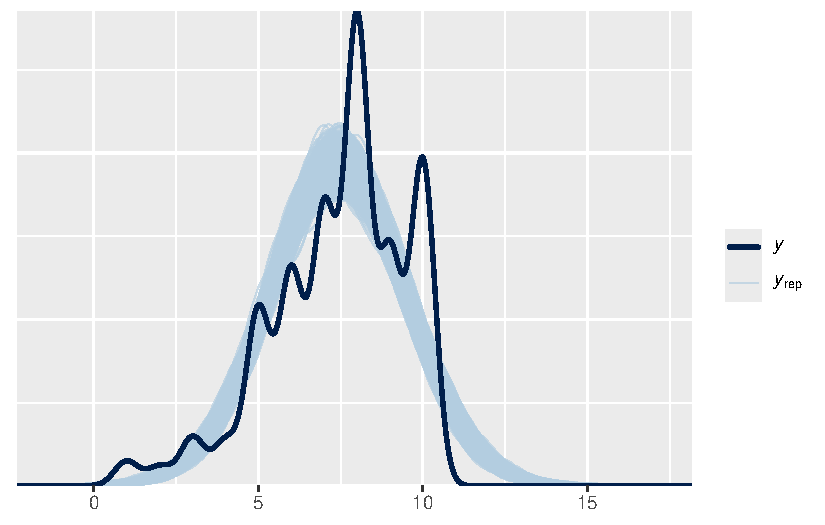
\includegraphics{paper_files/figure-pdf/fig-checks-1.pdf}

}

\caption{\label{fig-checks-1}Happiness Model Checks}

\end{figure}

\begin{figure}

{\centering \includegraphics{paper_files/figure-pdf/fig-checks-2.pdf}

}

\caption{\label{fig-checks-2}Happiness Model Checks}

\end{figure}

The posterior predictive check, visualized by \textbf{?@fig-checks},
helps us evaluate the fit of our Bayesian model. By overlapping the
observed happiness data with the simulated posterior predictive values,
this plot illustrates how well our model reproduces the observed
outcomes. The congruence between the values signifies that the model
adequately captures the central tendency and variability of the actual
happiness scores. Notably, if there are significant deviations it could
indicate that the model may not fully account for the data's
characteristics, prompting us to consider model refinements or
additional predictors.

The trace plot provides a representation of the Markov Chain Monte Carlo
(MCMC) sampling process, essential for evaluating the convergence of the
chains. Each parameter's trace, represented by individual lines for each
chain, should display a ``mixing'' behavior, converging to and
fluctuating around a common value, without exhibiting trends or
periodicity. Such patterns indicate that the chains have reached a
stationary distribution, and the samples drawn are likely from the true
posterior distribution. If the chains do not converge, this implies that
the sampling process has not yet adequately captured the full behaviour
of the true distribution, and further iterations or model adjustments
may be required to ensure reliable inference.

\hypertarget{discussion-sec-discussion}{%
\section{\texorpdfstring{Discussion
\{\textbf{?@sec-discussion}\}}{Discussion \{?@sec-discussion\}}}\label{discussion-sec-discussion}}

\hypertarget{sec-first-point}{%
\subsection{Model Findings}\label{sec-first-point}}

As shown in our \textbf{?@sec-results} section, we found that the
initial baseline measure for happiness in China was quite high, at a
predicted level of 7.60 given all other variables are at zero. We
discover that our results disagree with Helliwell and Putnam's (2004)
findings where belief in government policies are positively correlated
with well-being. Our model suggests that an increase in support for any
of the three policies correlates with a slight decrease in overall
happiness level. However, we find that although national pride is
negatively correlated with our measure of happiness, once we factor in
that national pride is measured on a scale of 1-5 with 1 being the
highest, we realize that national pride is the largest indicator of
happiness out of our chosen variables. This could be because we are
exclusively looking at a population of Chinese citizens. It is expected
that residents and citizens that do not pride themselves in being
Chinese are generally less happy while they are living there.
Furthermore, we see a very slight positive coefficient for our age
variable, suggesting that as Chinese citizens grow, they become more
satisfied with their life. This could be potentially attributed to the
stressful career and educational lifestyle of China. With a culture of
overworking compounded with the pressure of the Gaokao, young citizens
may experience lower levels of overall happiness compared to the older
generation.

From our results, we see that even with growing discontentment towards
China in the Western world, national pride and happiness levels seem to
be unhindered and remain reasonably high. Yet, we also notice support
for overreaching government policies with regards to surveillance and
monitoring does not correlate with the high levels of national pride.
Therefore, it is reasonable to conclude that although most Chinese
citizens are very proud of their nationality, that does not necessarily
correspond with support for the actions of the government.

\hypertarget{weaknesses-and-next-steps}{%
\subsection{Weaknesses and next steps}\label{weaknesses-and-next-steps}}

With an R-squared value of 0.048, it seems that an incredibly small
amount of variance is explained by our model. This is most likely due to
omitted variable bias, where we neglected to include several other
important factors when developing our regression model. Therefore, it is
very likely that our chosen variables on support for government policies
and/or national pride are not that significant in predicting overall
happiness level. However, when considering the fact that the original
questionnaire contained approximately 300 questions, it is to be
expected that there would be a lot of unaccounted for variance in our
data. Perhaps stronger expected indicators of overall happiness would
consist marital status, annual income, and employment status. With
regards to our model, we would likely get a more accurate regression by
including more questions. However, due to the incredibly large amount of
questions and responses, this could lead to overfitting. Although the
adjusted R-squared value accounts partly for too many regressors, there
is no feasible way to run a Bayesian regression model on all 300
questions. Therefore, future iterations of this study could look at
combining several values into one. For example, support for government
surveillance could be combined into one variable instead of three
separate ones. Furthermore, questions that seem to have no impact on
happiness level could also be ommitted by user discretion.

Future research may also consist of comparisons between different
nations that partook in the World Values Survey. Specifically,
comparisons for national pride and government support between communist
and democratic countries may lead to interesting inferences on the
societal beliefs for their respective nations. A heavier reliance on
governmental structures in a communist society may lead to higher levels
of national pride when compared to less reliant democratic nations.

\newpage

\appendix

\hypertarget{appendix-sec-appendix}{%
\section{\texorpdfstring{Appendix
\{\textbf{?@sec-appendix}\}}{Appendix \{?@sec-appendix\}}}\label{appendix-sec-appendix}}

\begin{figure}

{\centering \includegraphics{paper_files/figure-pdf/fig-compiled-1.pdf}

}

\caption{\label{fig-compiled}Support for Surveillance, Email Monitoring,
and Information Collection by Age Group}

\end{figure}

\newpage

\hypertarget{references}{%
\section*{References}\label{references}}
\addcontentsline{toc}{section}{References}

\hypertarget{refs}{}
\begin{CSLReferences}{1}{0}
\leavevmode\vadjust pre{\hypertarget{ref-rstanarm}{}}%
Goodrich, Ben, Jonah Gabry, Imad Ali, and Sam Brilleman. 2022.
{``Rstanarm: {Bayesian} Applied Regression Modeling via {Stan}.''}
\url{https://mc-stan.org/rstanarm/}.

\leavevmode\vadjust pre{\hypertarget{ref-citeR}{}}%
R Core Team. 2023. \emph{R: A Language and Environment for Statistical
Computing}. Vienna, Austria: R Foundation for Statistical Computing.
\url{https://www.R-project.org/}.

\end{CSLReferences}



\end{document}
